\documentclass[12pt,a4paper]{article}

\usepackage[margin=2.5cm]{geometry}
\usepackage[utf8]{inputenc}
\usepackage[brazil]{babel}
\usepackage{lmodern}
\usepackage{fancyhdr}
\usepackage{tocloft}
\usepackage{amsmath}
\usepackage{graphicx}
\usepackage{booktabs}
\usepackage{array}
\usepackage{float}
\usepackage{hyperref}
\usepackage{lastpage}
\usepackage{subcaption}
\usepackage{multirow}

\graphicspath{{../../../imagens_gerais/} {images/}} 

\pagestyle{fancy}
\fancyhf{} 
\setlength{\headheight}{30pt}
\lhead{
  \includegraphics[height=1.2cm]{lafe_logo_ingles.jpg} \\
  \small
  Doc ID: PLT0074 \quad
  Doc tipo: Relatório de fabricação \quad
}
\rhead{
  \small \textbf{PLT0074 Suspended core em PETG esverdeado} \\
  Page \thepage\ of \pageref{LastPage}
}
\lfoot{\small \textcopyright\ 2026 LaFE. All rights reserved.}
\rfoot{\small Última data de revisão: 17/07/2026}

\begin{document}

  Descrição da participação dos envolvidos na fabricação desta fibra:
  \begin{itemize}
    \item Ivan Prearo: Fabricação e puxamento
  \end{itemize}

  \section*{Puxamento}
  \label{sec:puxamento}

Este puxamento é de uma preforma do tipo \textit{hollow-core} com dimensões mostradas na Tabela \ref{tab:medidas_preforma}, com a notação de cada dimensão mostrada na Fig \ref{fig:dimensoes_preforma}.
A preforma é mostrada na Figura \ref{fig:foto_preforma}, e tem microestrutura \textit{hollow-core} da Figura \ref{fig:desenho_preforma}.

  \begin{table}[H]
    \centering
	  \begin{tabular}{ccc}	
		  \textbf{Medida} & \textbf{Medida absoluta [mm]} & \textbf{Medida relativa} \\ 
		  \hline
		  $\phi_{out}$ & 15 & 1.000 \\
		  $L_{out}$ & 2.5 & 0.167 \\
      $\phi_{in}$ & 1.45 & 0.097 \\
		  $L_{in}$ & 0.6 & 0.040 \\
      $d_{int}$ & 1 & 0.067
	  \end{tabular}
	  \caption{Medidas na preforma.}
	  \label{tab:medidas_preforma}
  \end{table}

\begin{figure}[H]
	\centering
  \begin{subfigure}[t]{0.4\linewidth}
    \centering
	  
\includegraphics[width=\linewidth]{Modelo.png}
    \caption{Seção transversal da preforma.}
    \label{fig:desenho_preforma}
  \end{subfigure}
  \begin{subfigure}[t]{0.4\linewidth}
    \centering
	  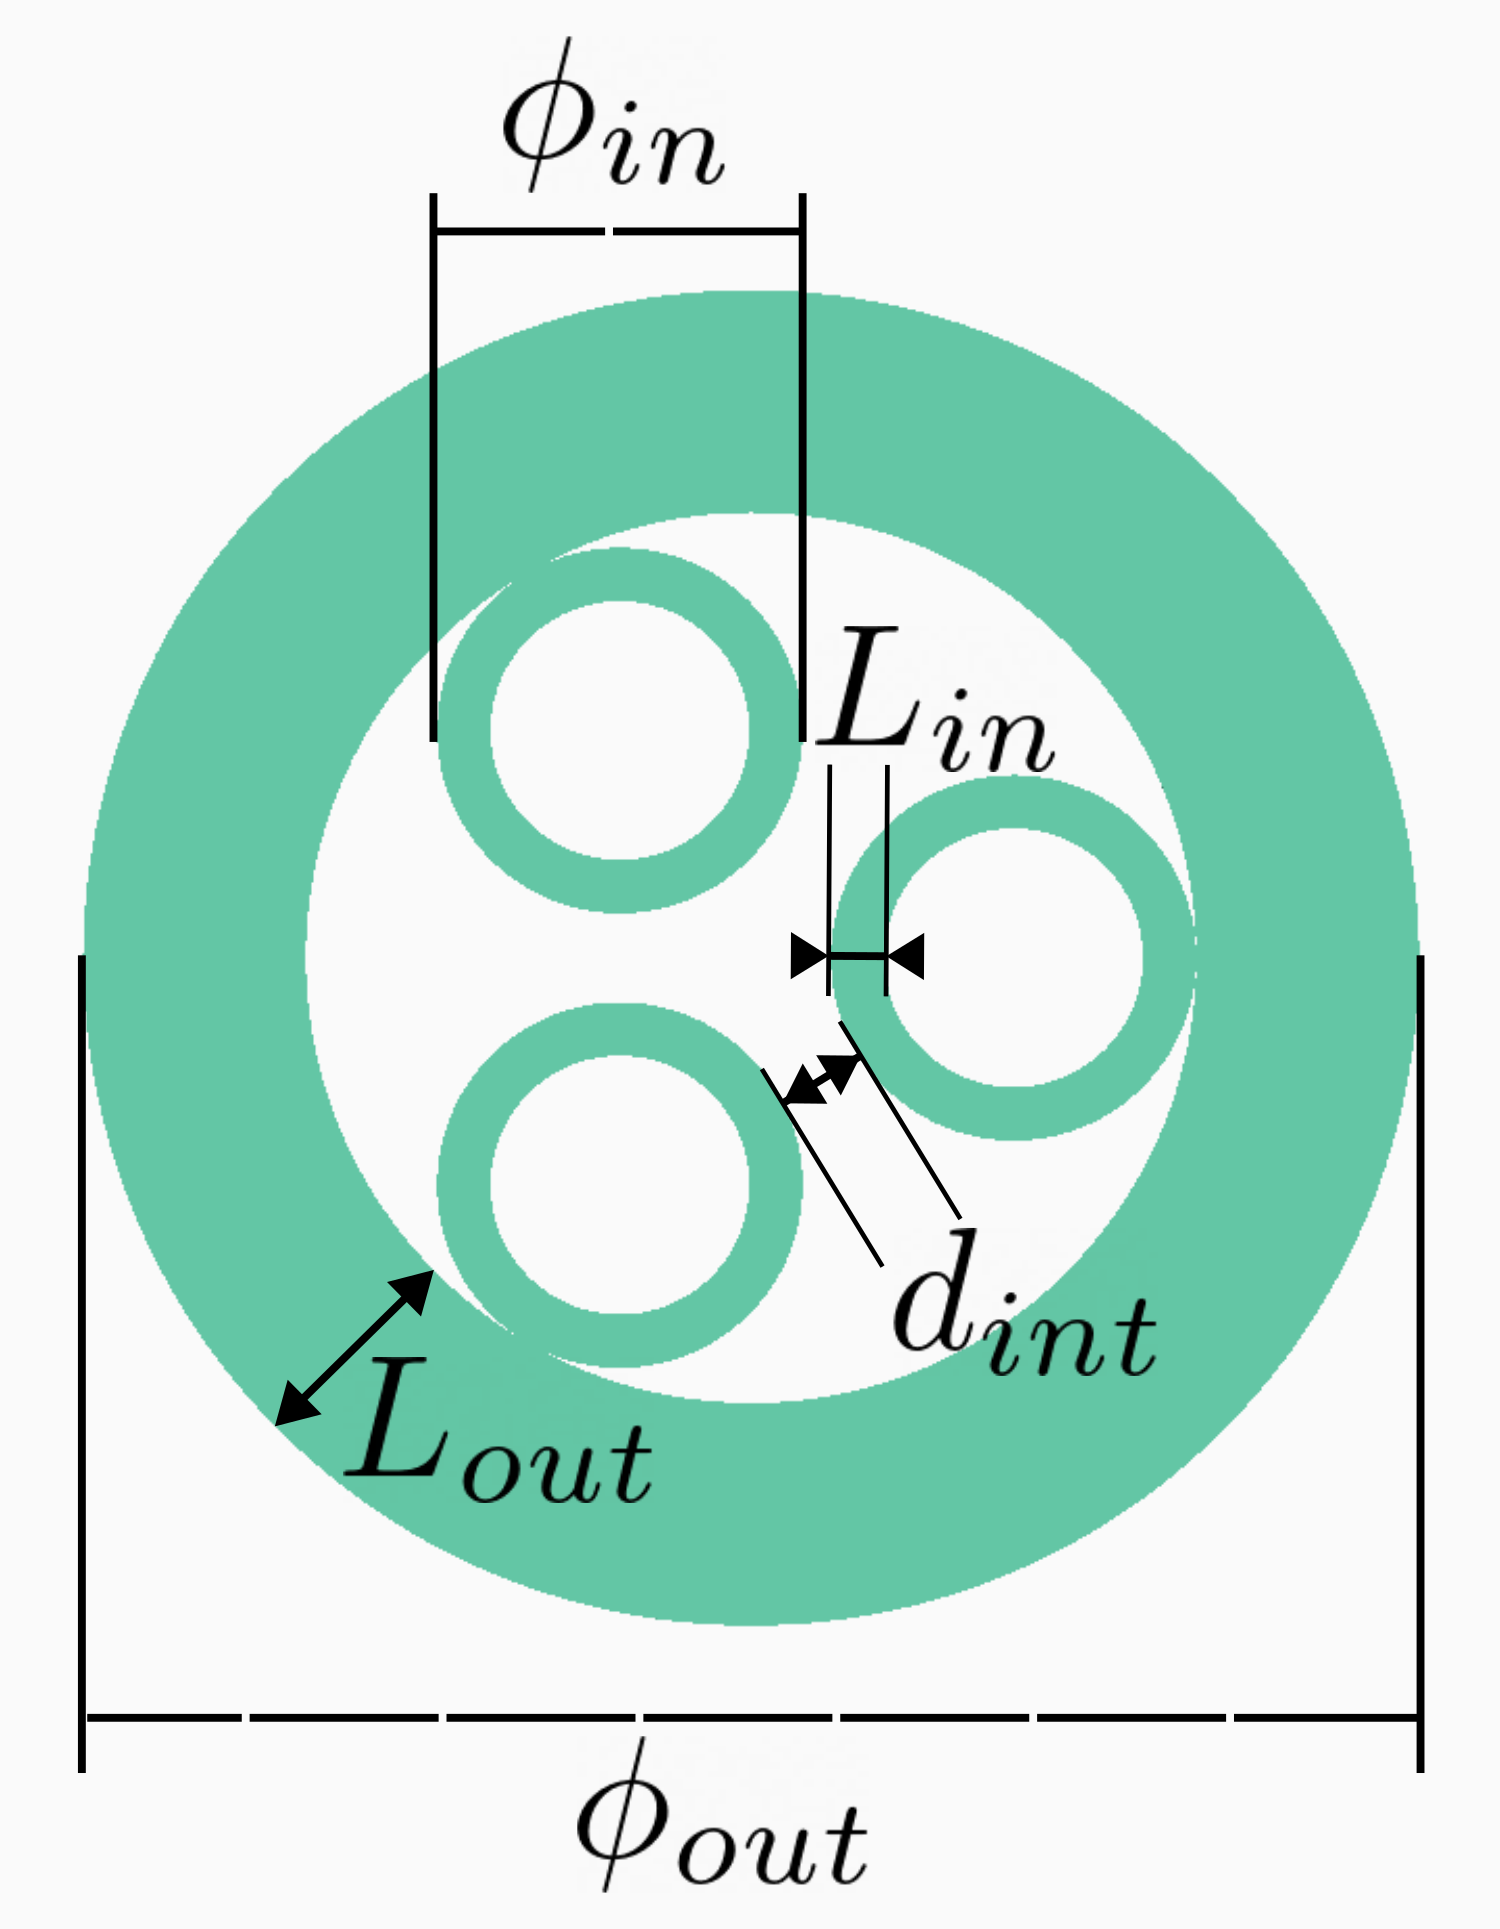
\includegraphics[height=\linewidth]{Dimensoes.png}
    \caption{Dimensões especificadas.}
    \label{fig:dimensoes_preforma}
  \end{subfigure}
  \begin{subfigure}[t]{0.15\linewidth}
    \centering
	  
\includegraphics[height=2.67\linewidth]{Preforma.jpeg}
    \caption{Preforma.}
    \label{fig:foto_preforma}
  \end{subfigure}
	\caption{Especificações da microestrutura desenhada. Desenhos em escala.}
	\label{fig:preforma}
\end{figure}


  Para realizar o puxamento utilizamos a rampa de temperatura descrita na Tabela \ref{tab:puxamento_rampa}.

\begin{table}[H]
  \centering
  \begin{tabular}{ccc}   
    \toprule 
    \textbf{Fase} & \textbf{[°C]} & \textbf{Tempo [min]} \\ 
    \midrule
    \multirow{2}{*}{Secagem} & 60 & 60 \\
                              & 80 & 15 \\
    \midrule
    \multirow{2}{*}{Escoamento} & 100 & 5 \\
                              & 110 & 2 \\ 
    \midrule
    \multirow{2}{*}{Puxamento} & 120 & 15 \\
                                & 123 & -- \\
    \midrule
    Puxamento (Capstan)        & 120 & -- \\
    \bottomrule
  \end{tabular}
  \caption{Rampa de temperatura no forno da torre antes e durante o puxamento.}
  \label{tab:puxamento_rampa}
\end{table}

\section*{Resultados}
\label{sec:resultados}

 Foram produzidos cerca de 17 metros de fibra com diâmetro externo entre 1 mm e 0.2 mm (Fig. \ref{fig:resultados_gerais}).
 Realizamos algumas microscopias para verificar a proporção da microestrutura na fibra final.
 Para isso, medimos as dimensões de cada atributo da fibra a fim de calcular a razão entre elas (Figura \ref{fig:secoes_transversais}).
 Ambas as micrografias da Figura \ref{fig:secoes_transversais} são da banda A, uma vez que o diâmetro da fibra na banda B era demasiado pequeno e não permitia clivagens razoáveis (Fig. \ref{fig:micrografia_banda_B}).
 Ainda, a microestrutura na fibra produzida estava irregular e portanto tomamos médias de diversas medições na mesma micrografia;
 por exemplo, medimos os diâmetros e larguras dos três capilares internos.
 Os diâmetros da fibra ao longo da fabricação estão graficados na Figura \ref{fig:grafico_diametros}.

  \begin{figure}[H]
    \centering
      \begin{subfigure}[t]{0.48\textwidth}
      \centering
      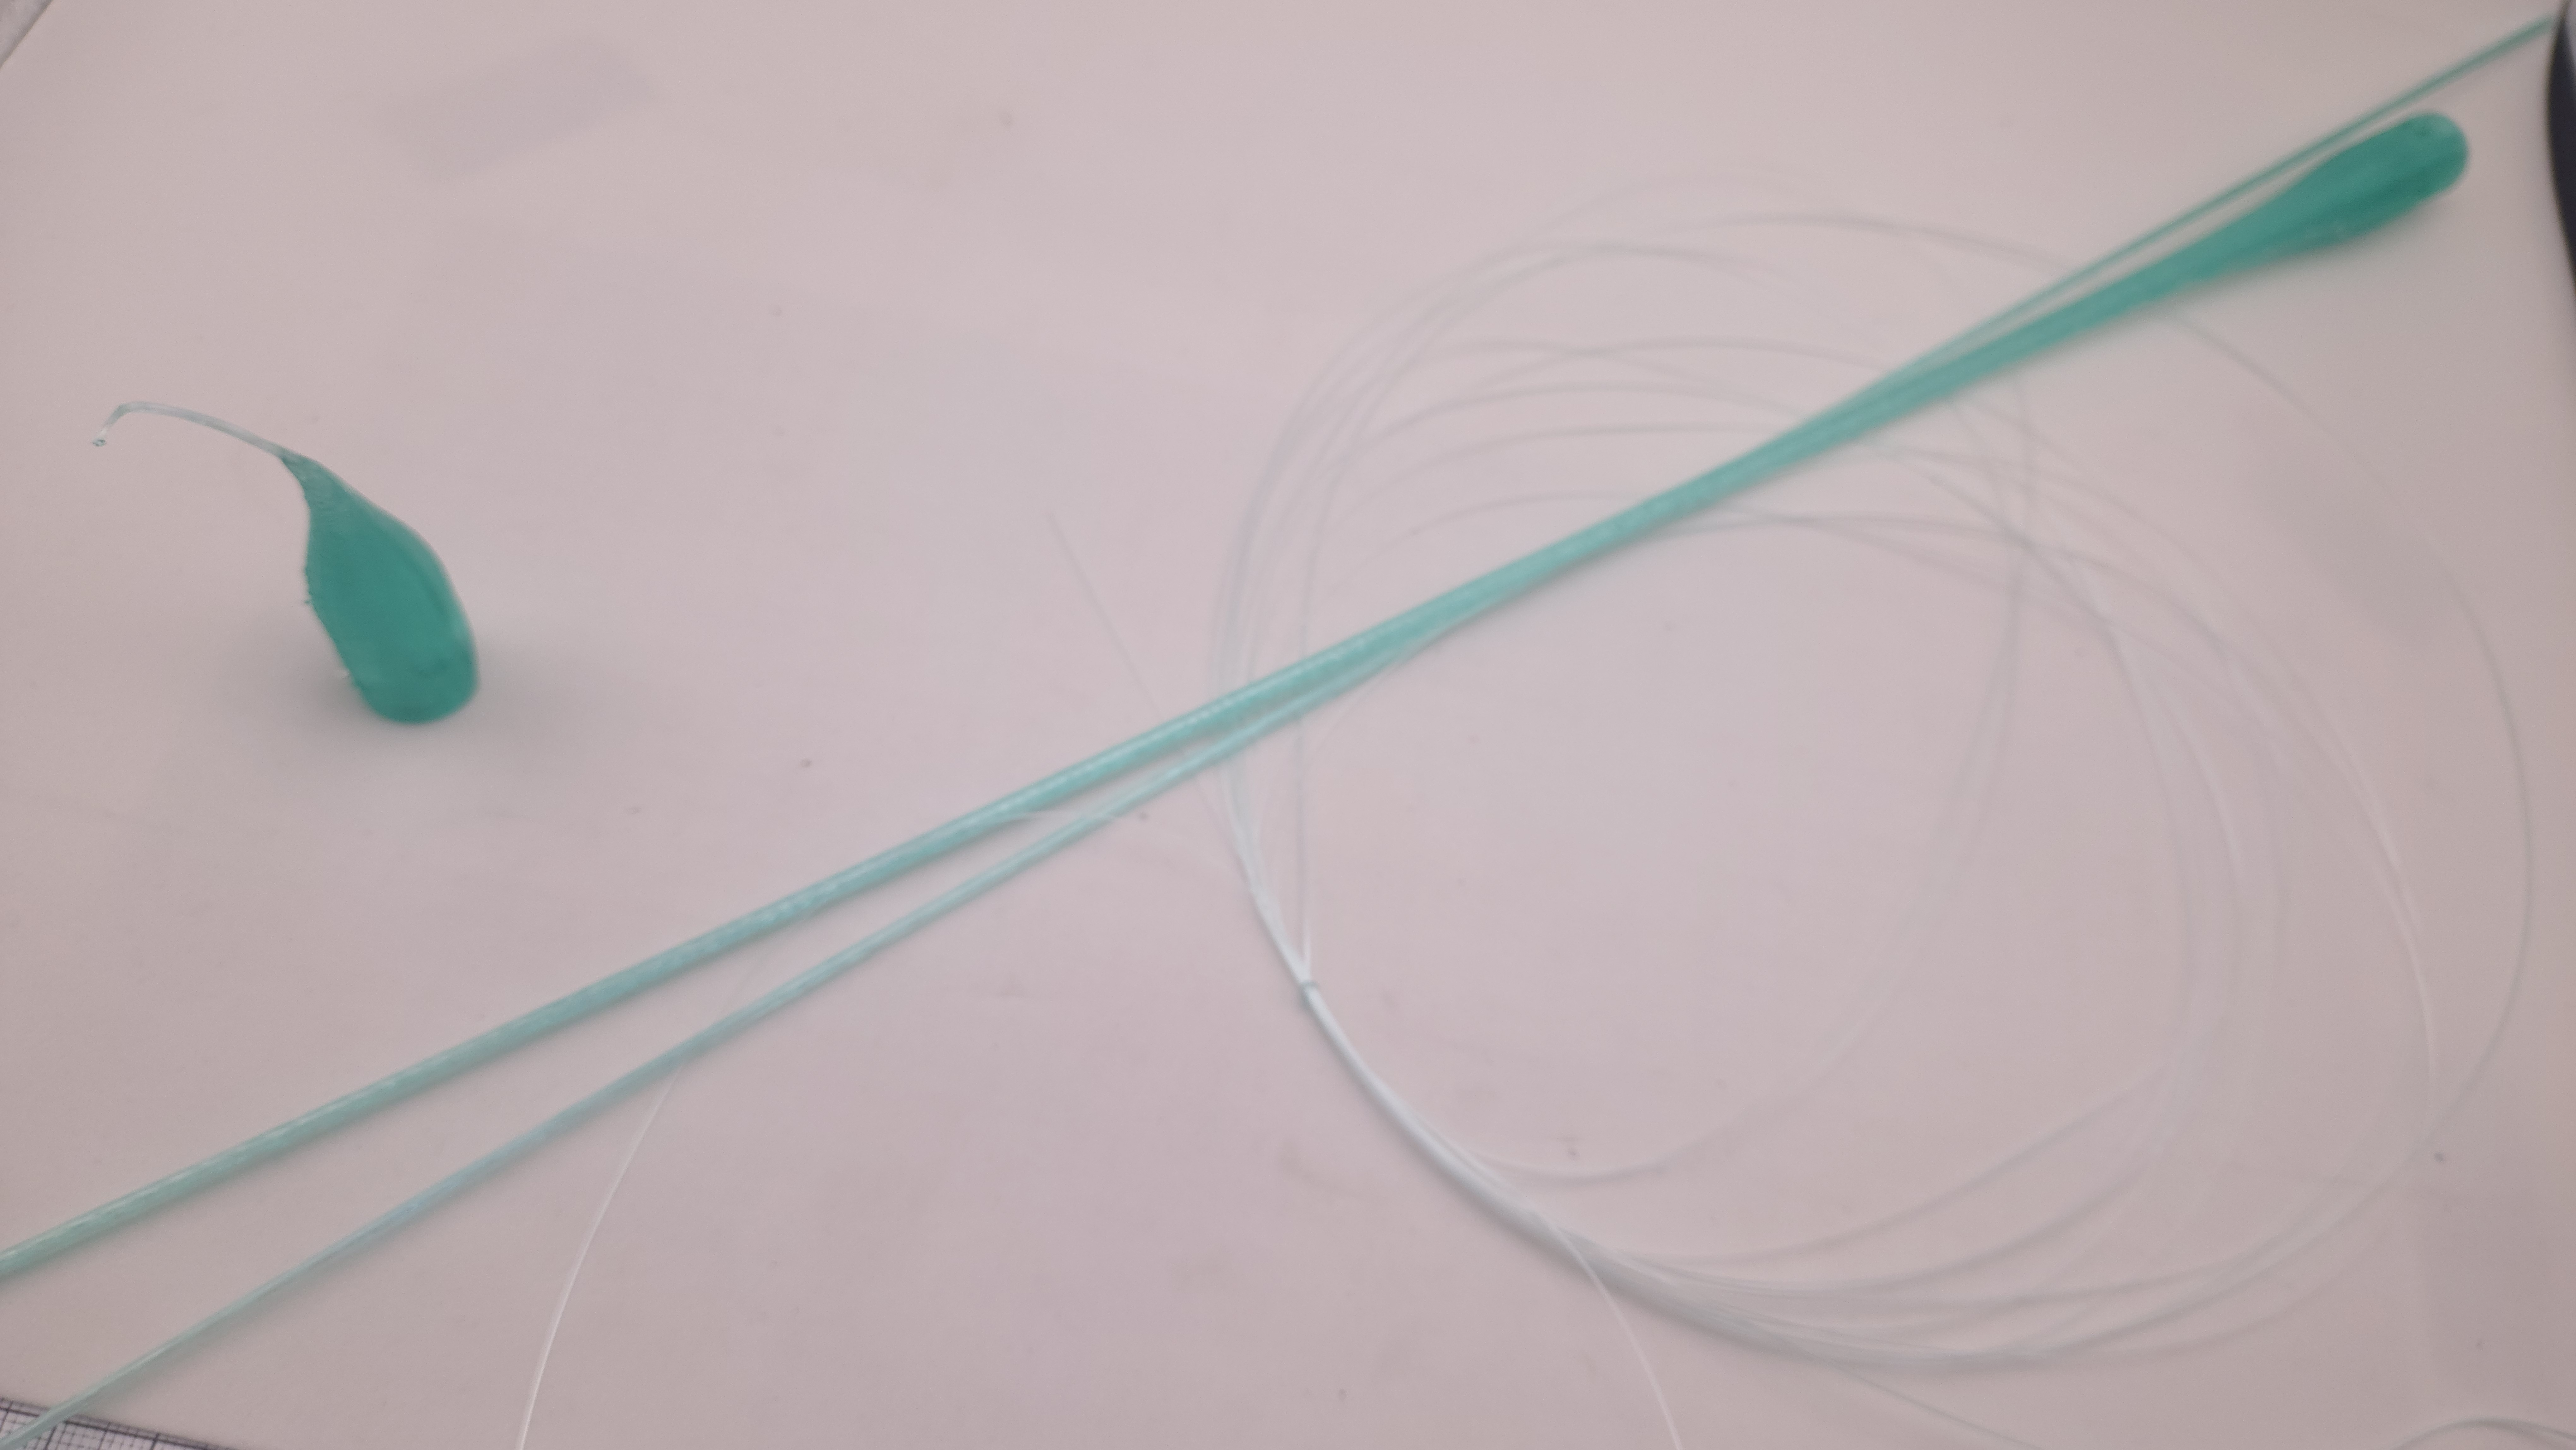
\includegraphics[width=1\linewidth]{Colecao_resultados.jpg}
      \caption{Resultados avulsos do puxamento.}
      \label{fig:colecao_resultados}
    \end{subfigure}
    \hfill
    \begin{subfigure}[t]{0.48\textwidth}
      \centering
      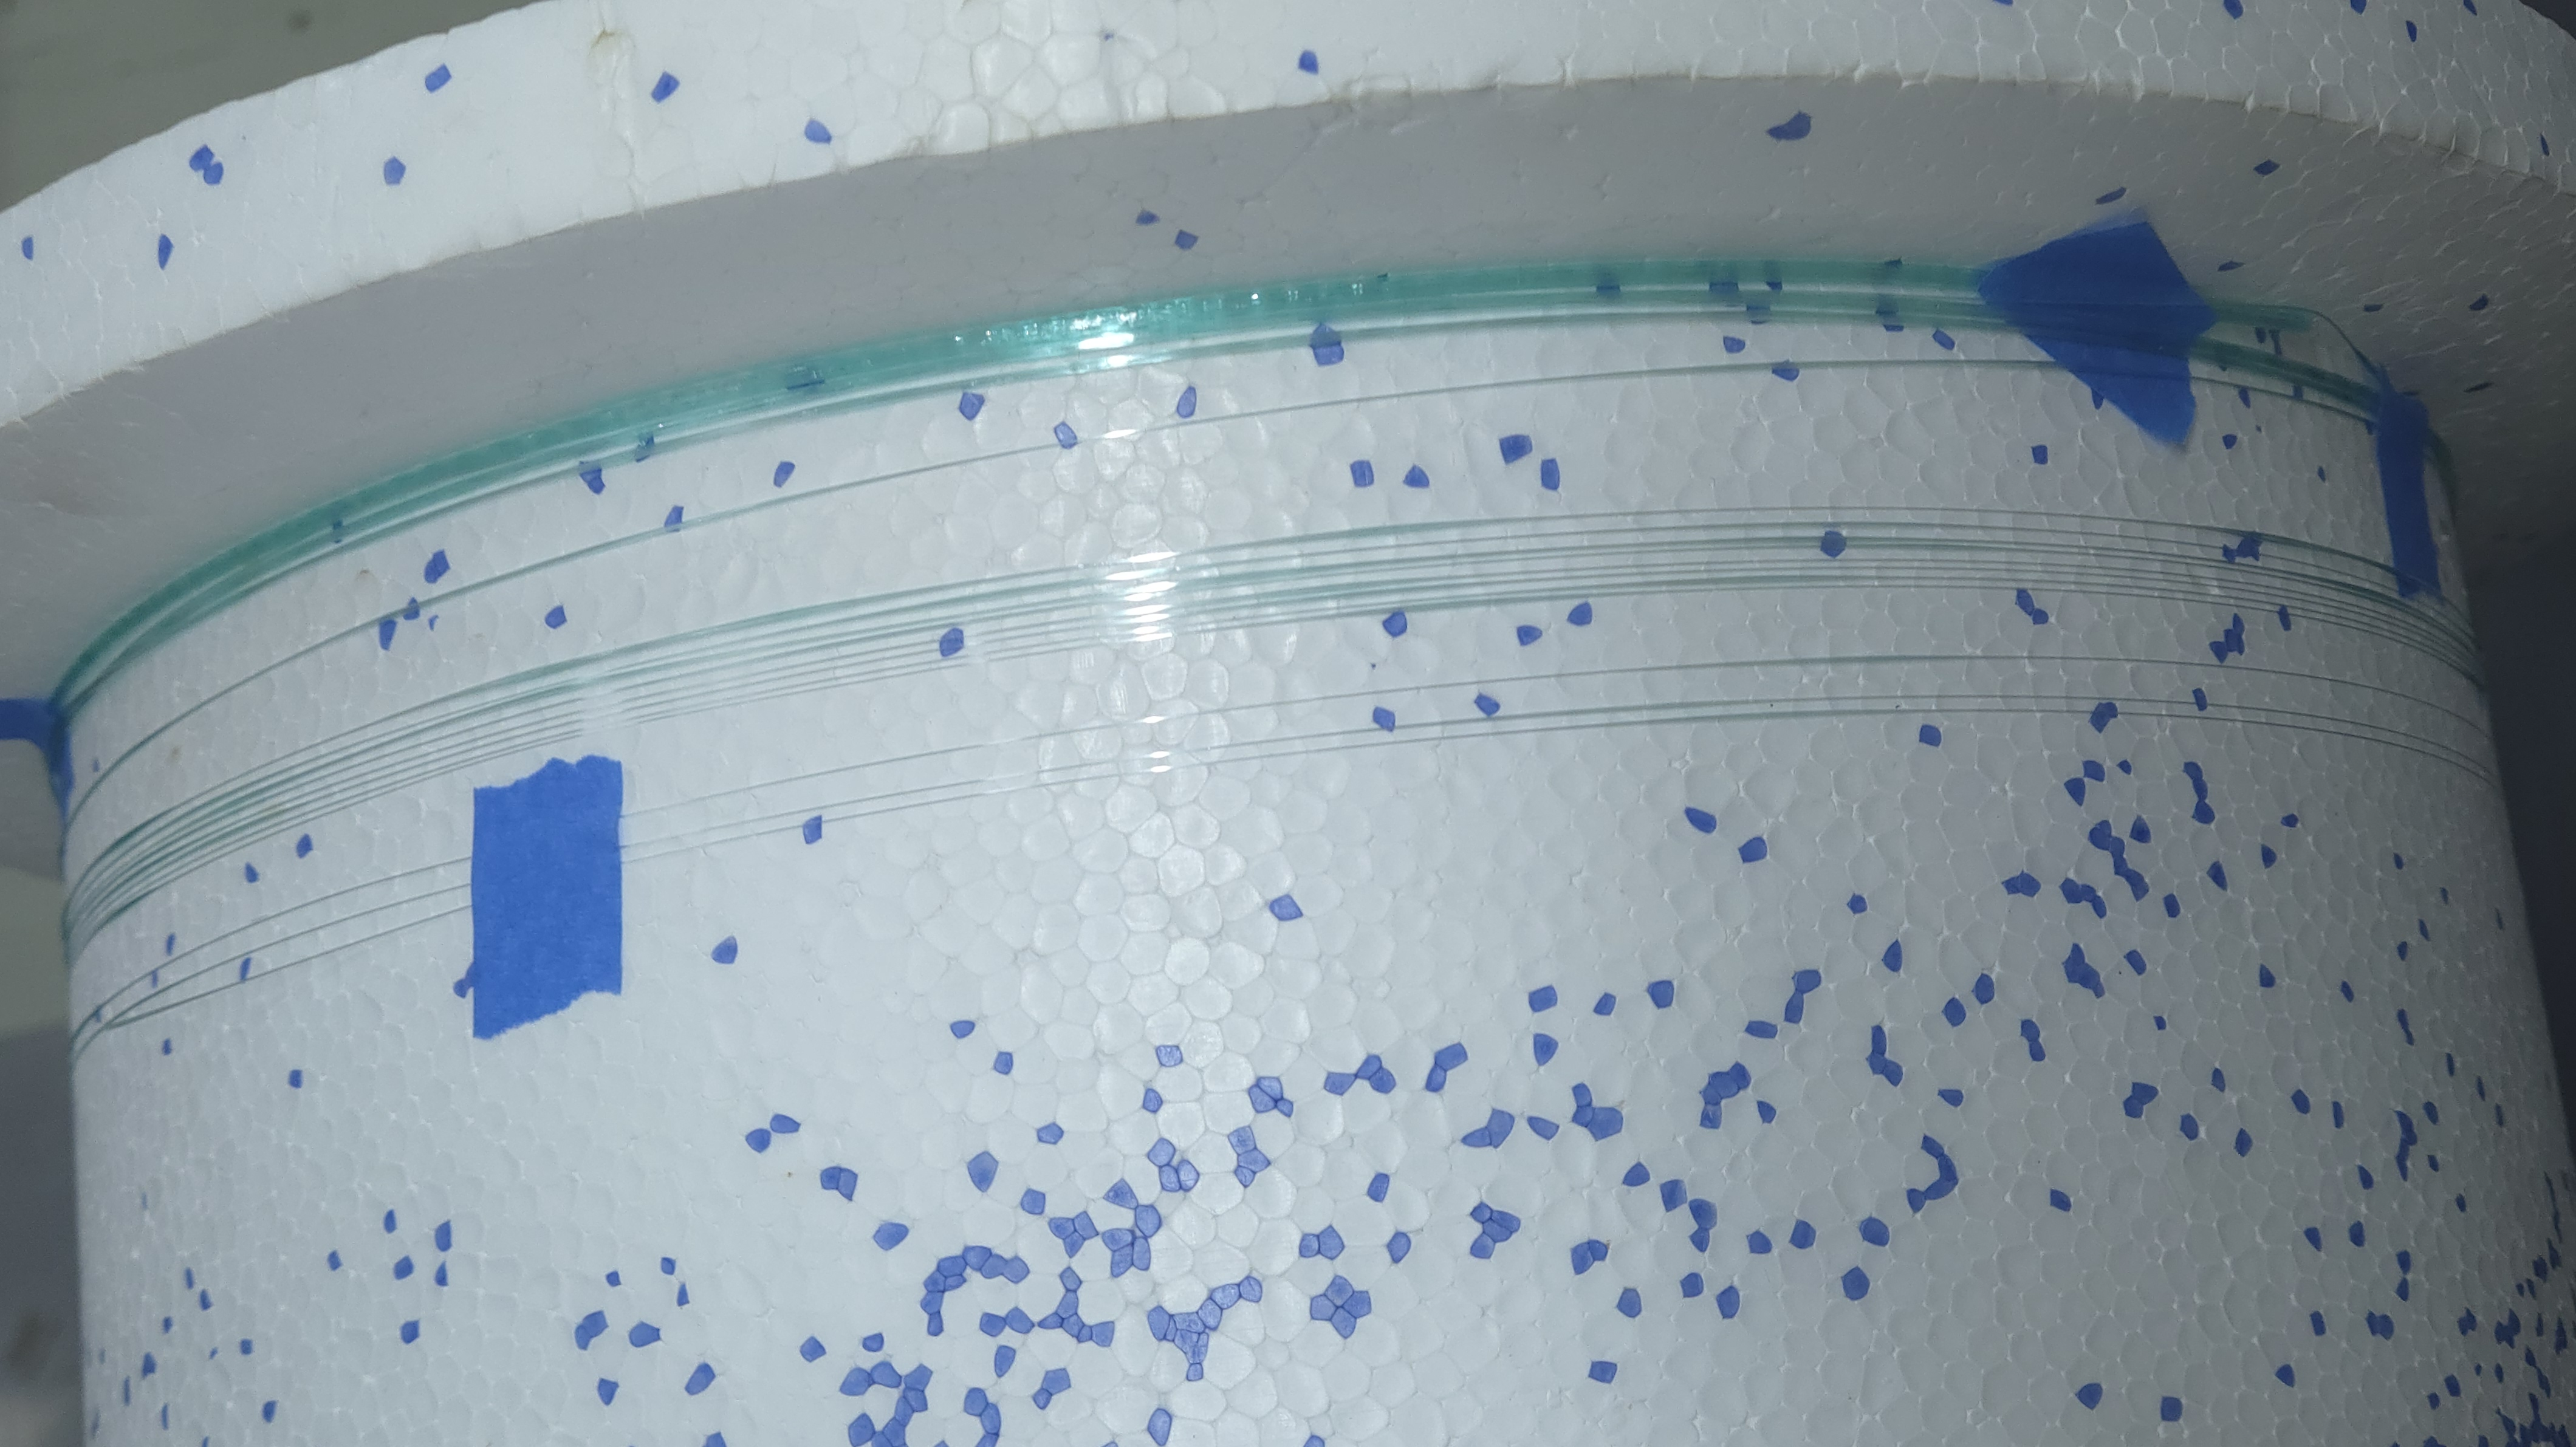
\includegraphics[width=1\linewidth]{Drum_resultados.jpg}
      \caption{Resultados do puxamento no \textit{drum winder}.}
      \label{fig:drum_resultados}
    \end{subfigure}
    \hfill
    \caption{Resultados do puxamento.}
    \label{fig:resultados_gerais}
  \end{figure}

  \begin{figure}[H]
    \centering
      \begin{subfigure}{0.45\textwidth}
      \centering
      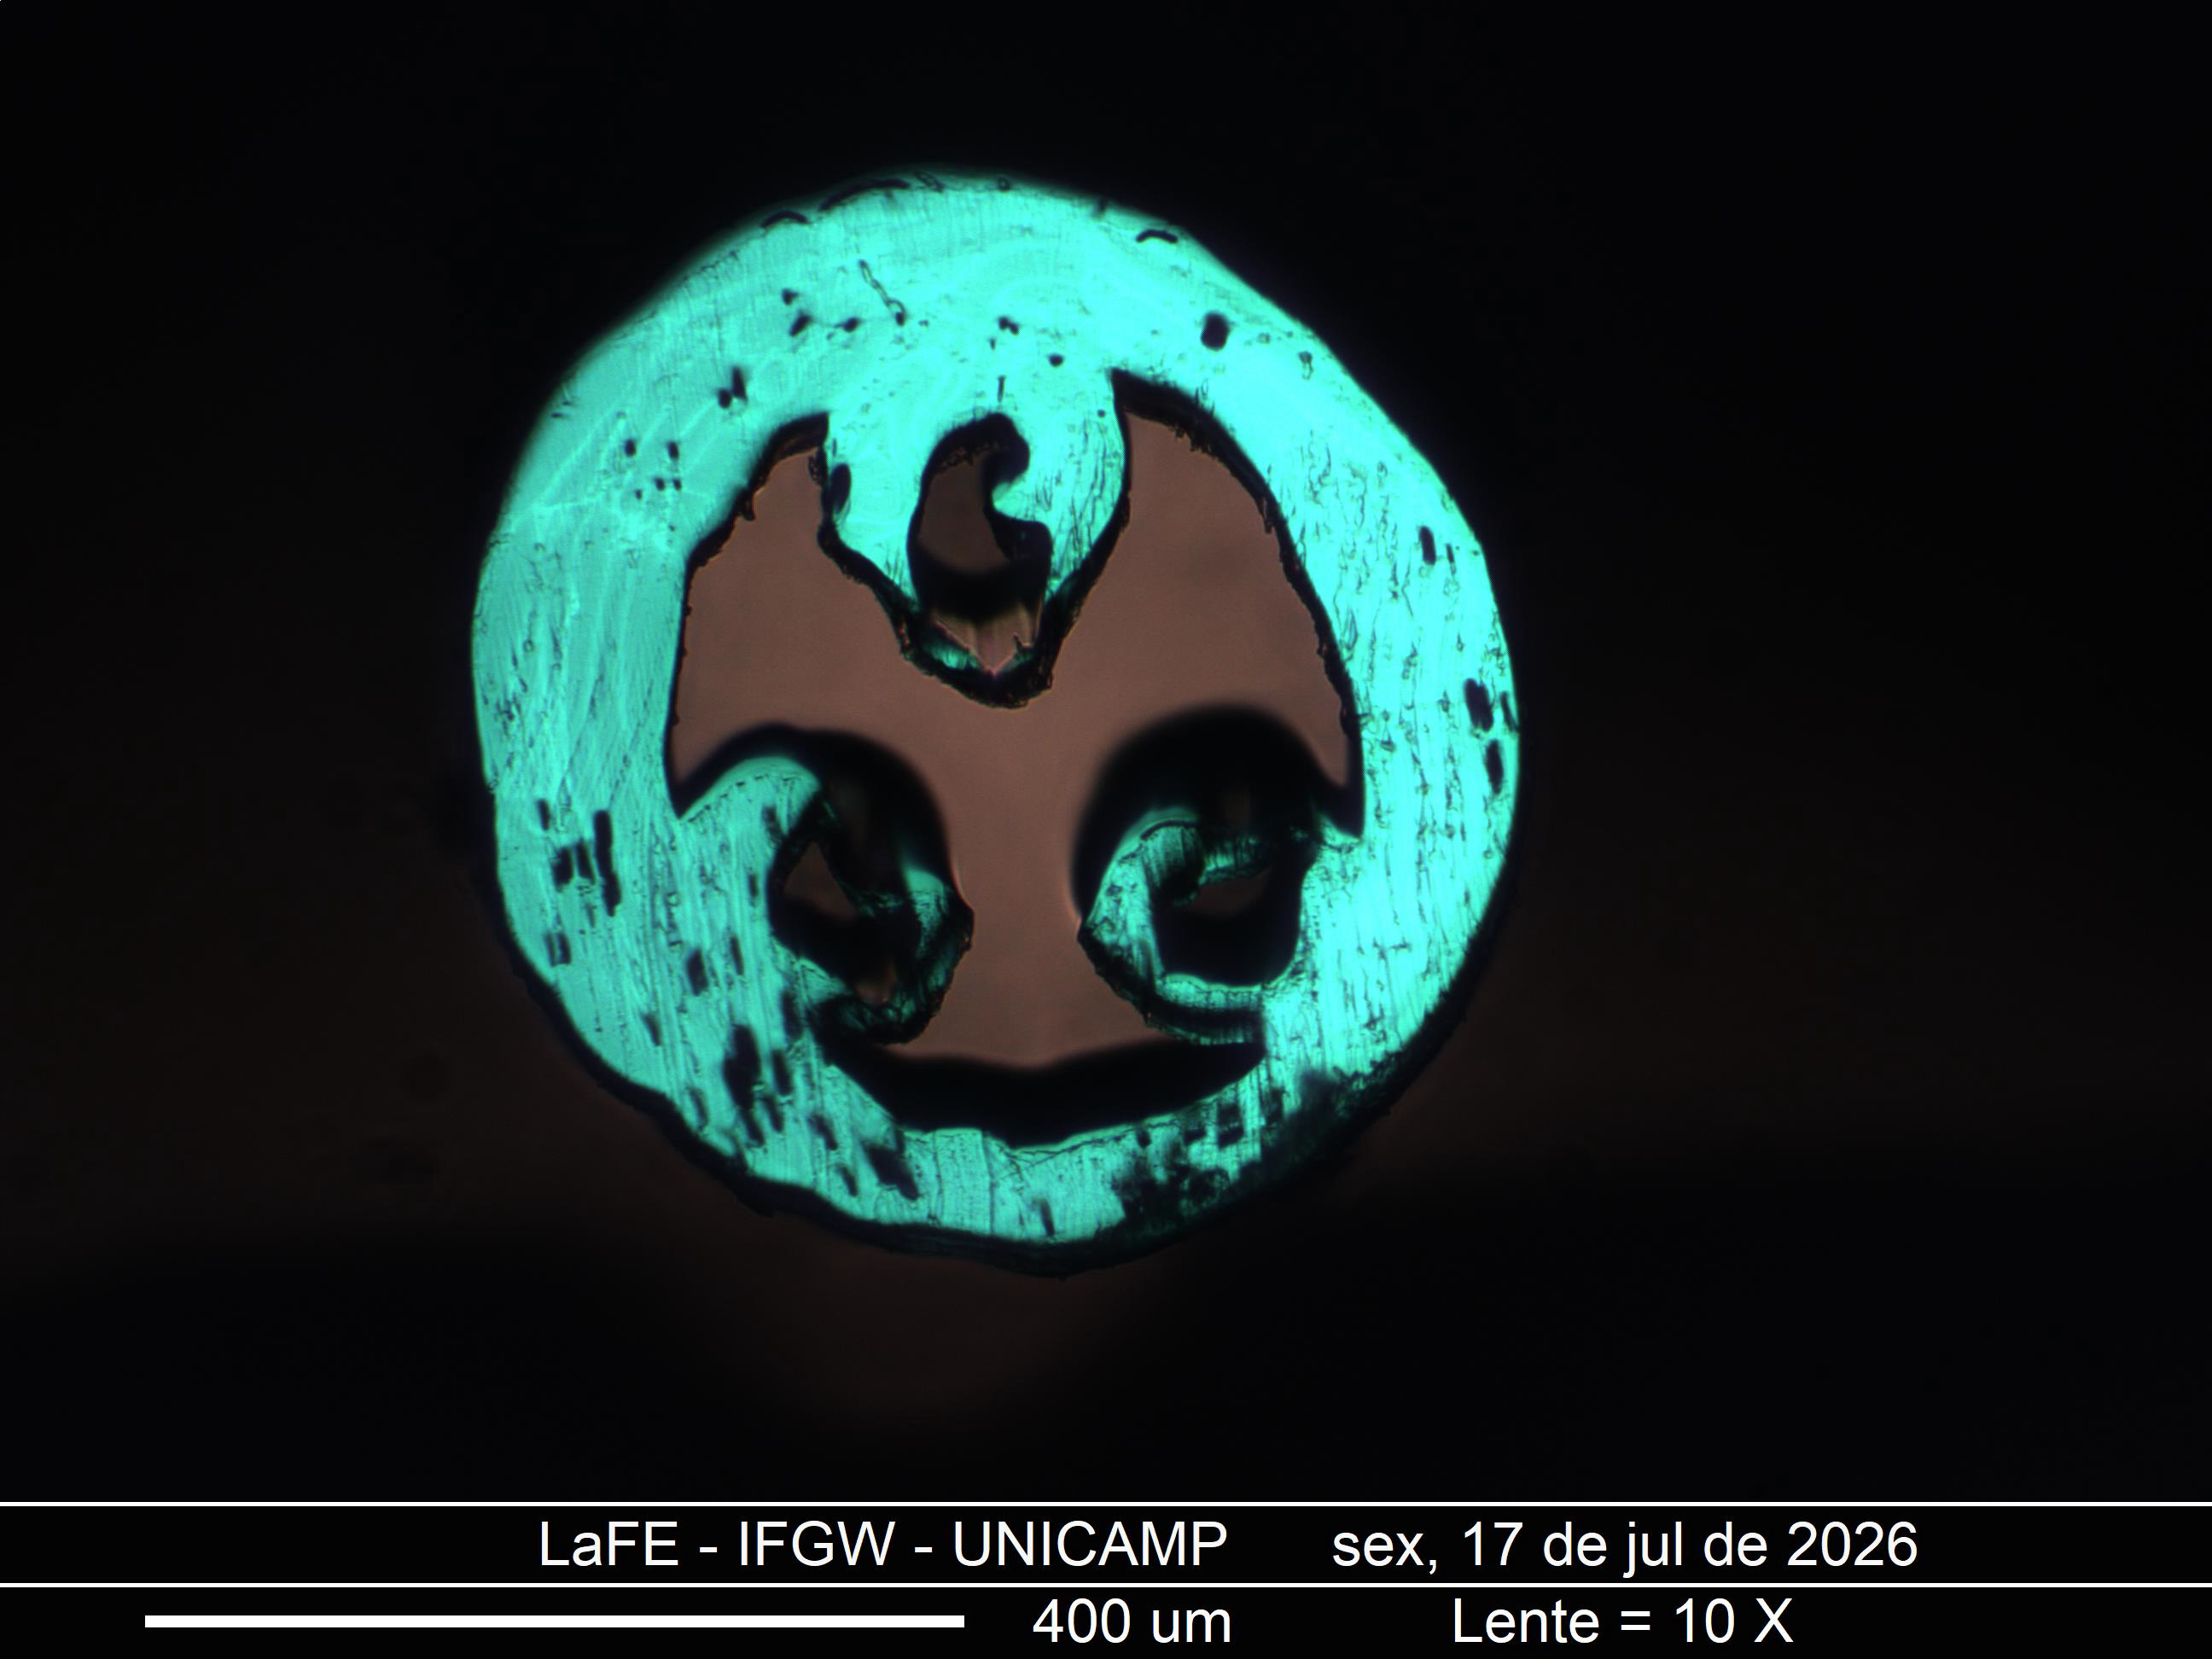
\includegraphics[width=1\linewidth]{Foto_M1.png}
      \caption{Micrografia M1.}
      \label{fig:micrografia_m1}
    \end{subfigure}
    \hfill
    \begin{subfigure}{0.45\textwidth}
      \centering
      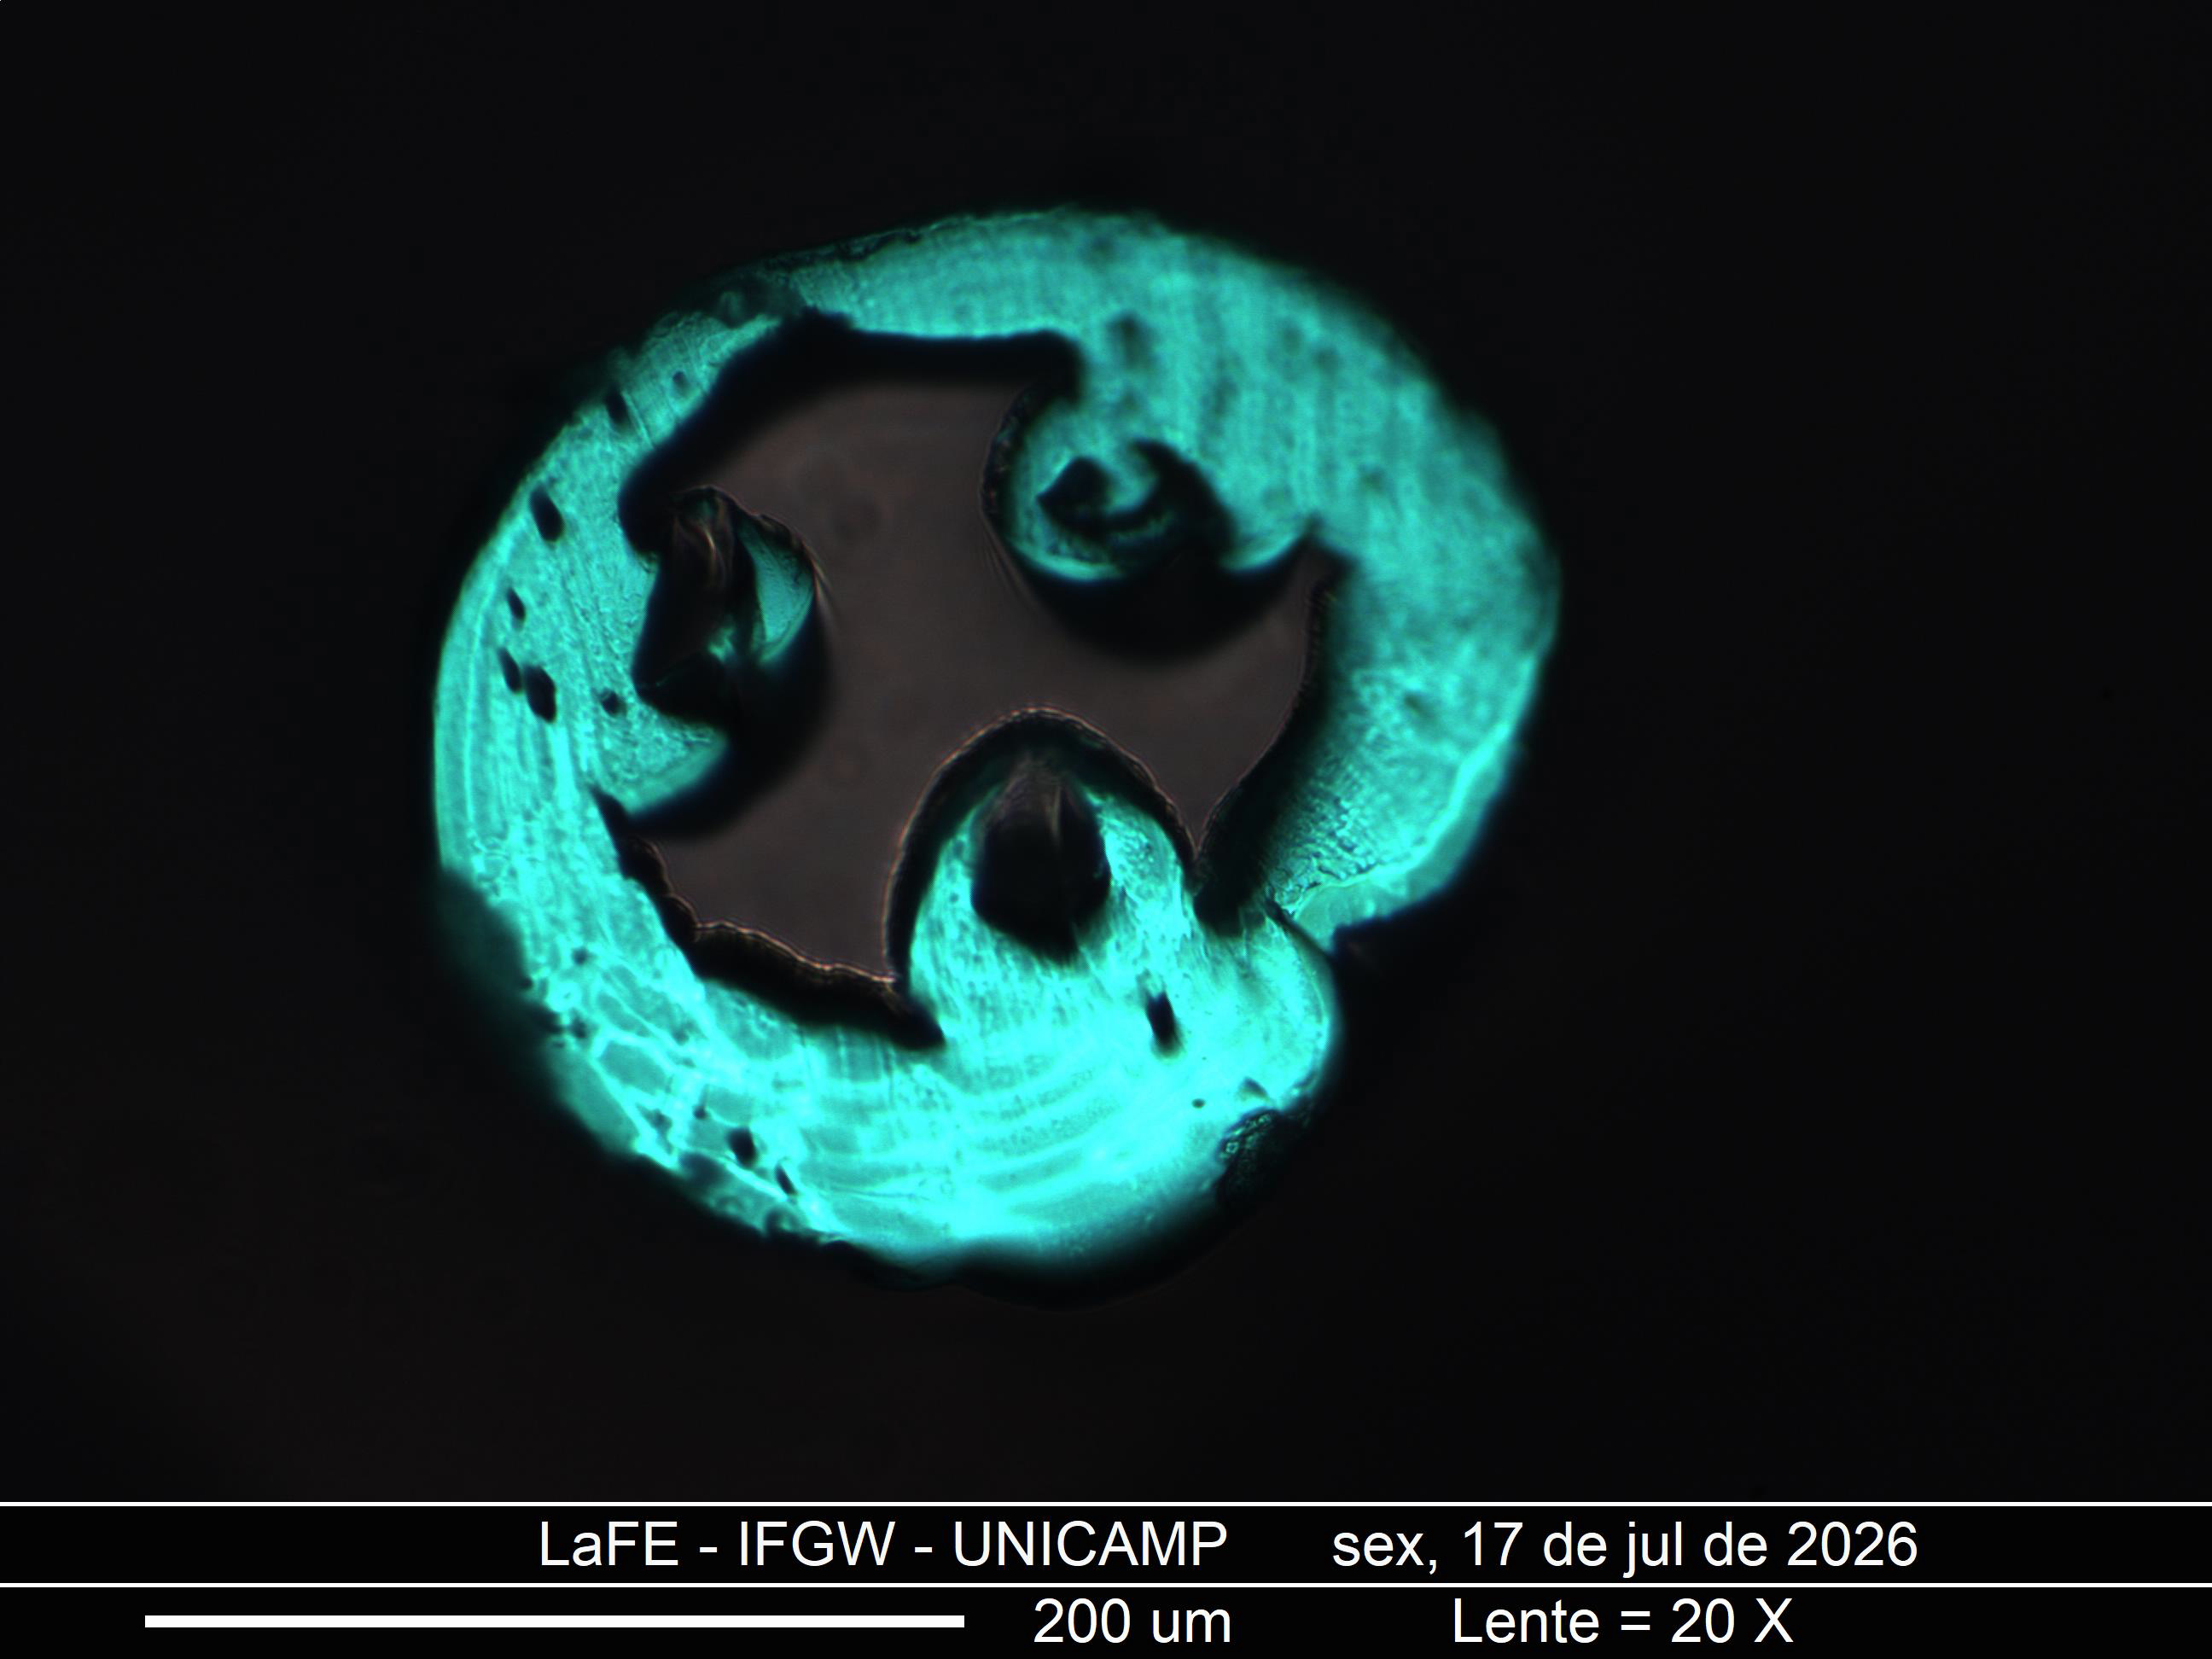
\includegraphics[width=1\linewidth]{Foto_M2.png}
      \caption{Micrografia M2.}
      \label{fig:micrografia_m2}
    \end{subfigure}
    \hfill
    \caption{Micrografias da banda A.}
    \label{fig:secoes_transversais}
  \end{figure}

  \begin{figure}[H]
    \centering
    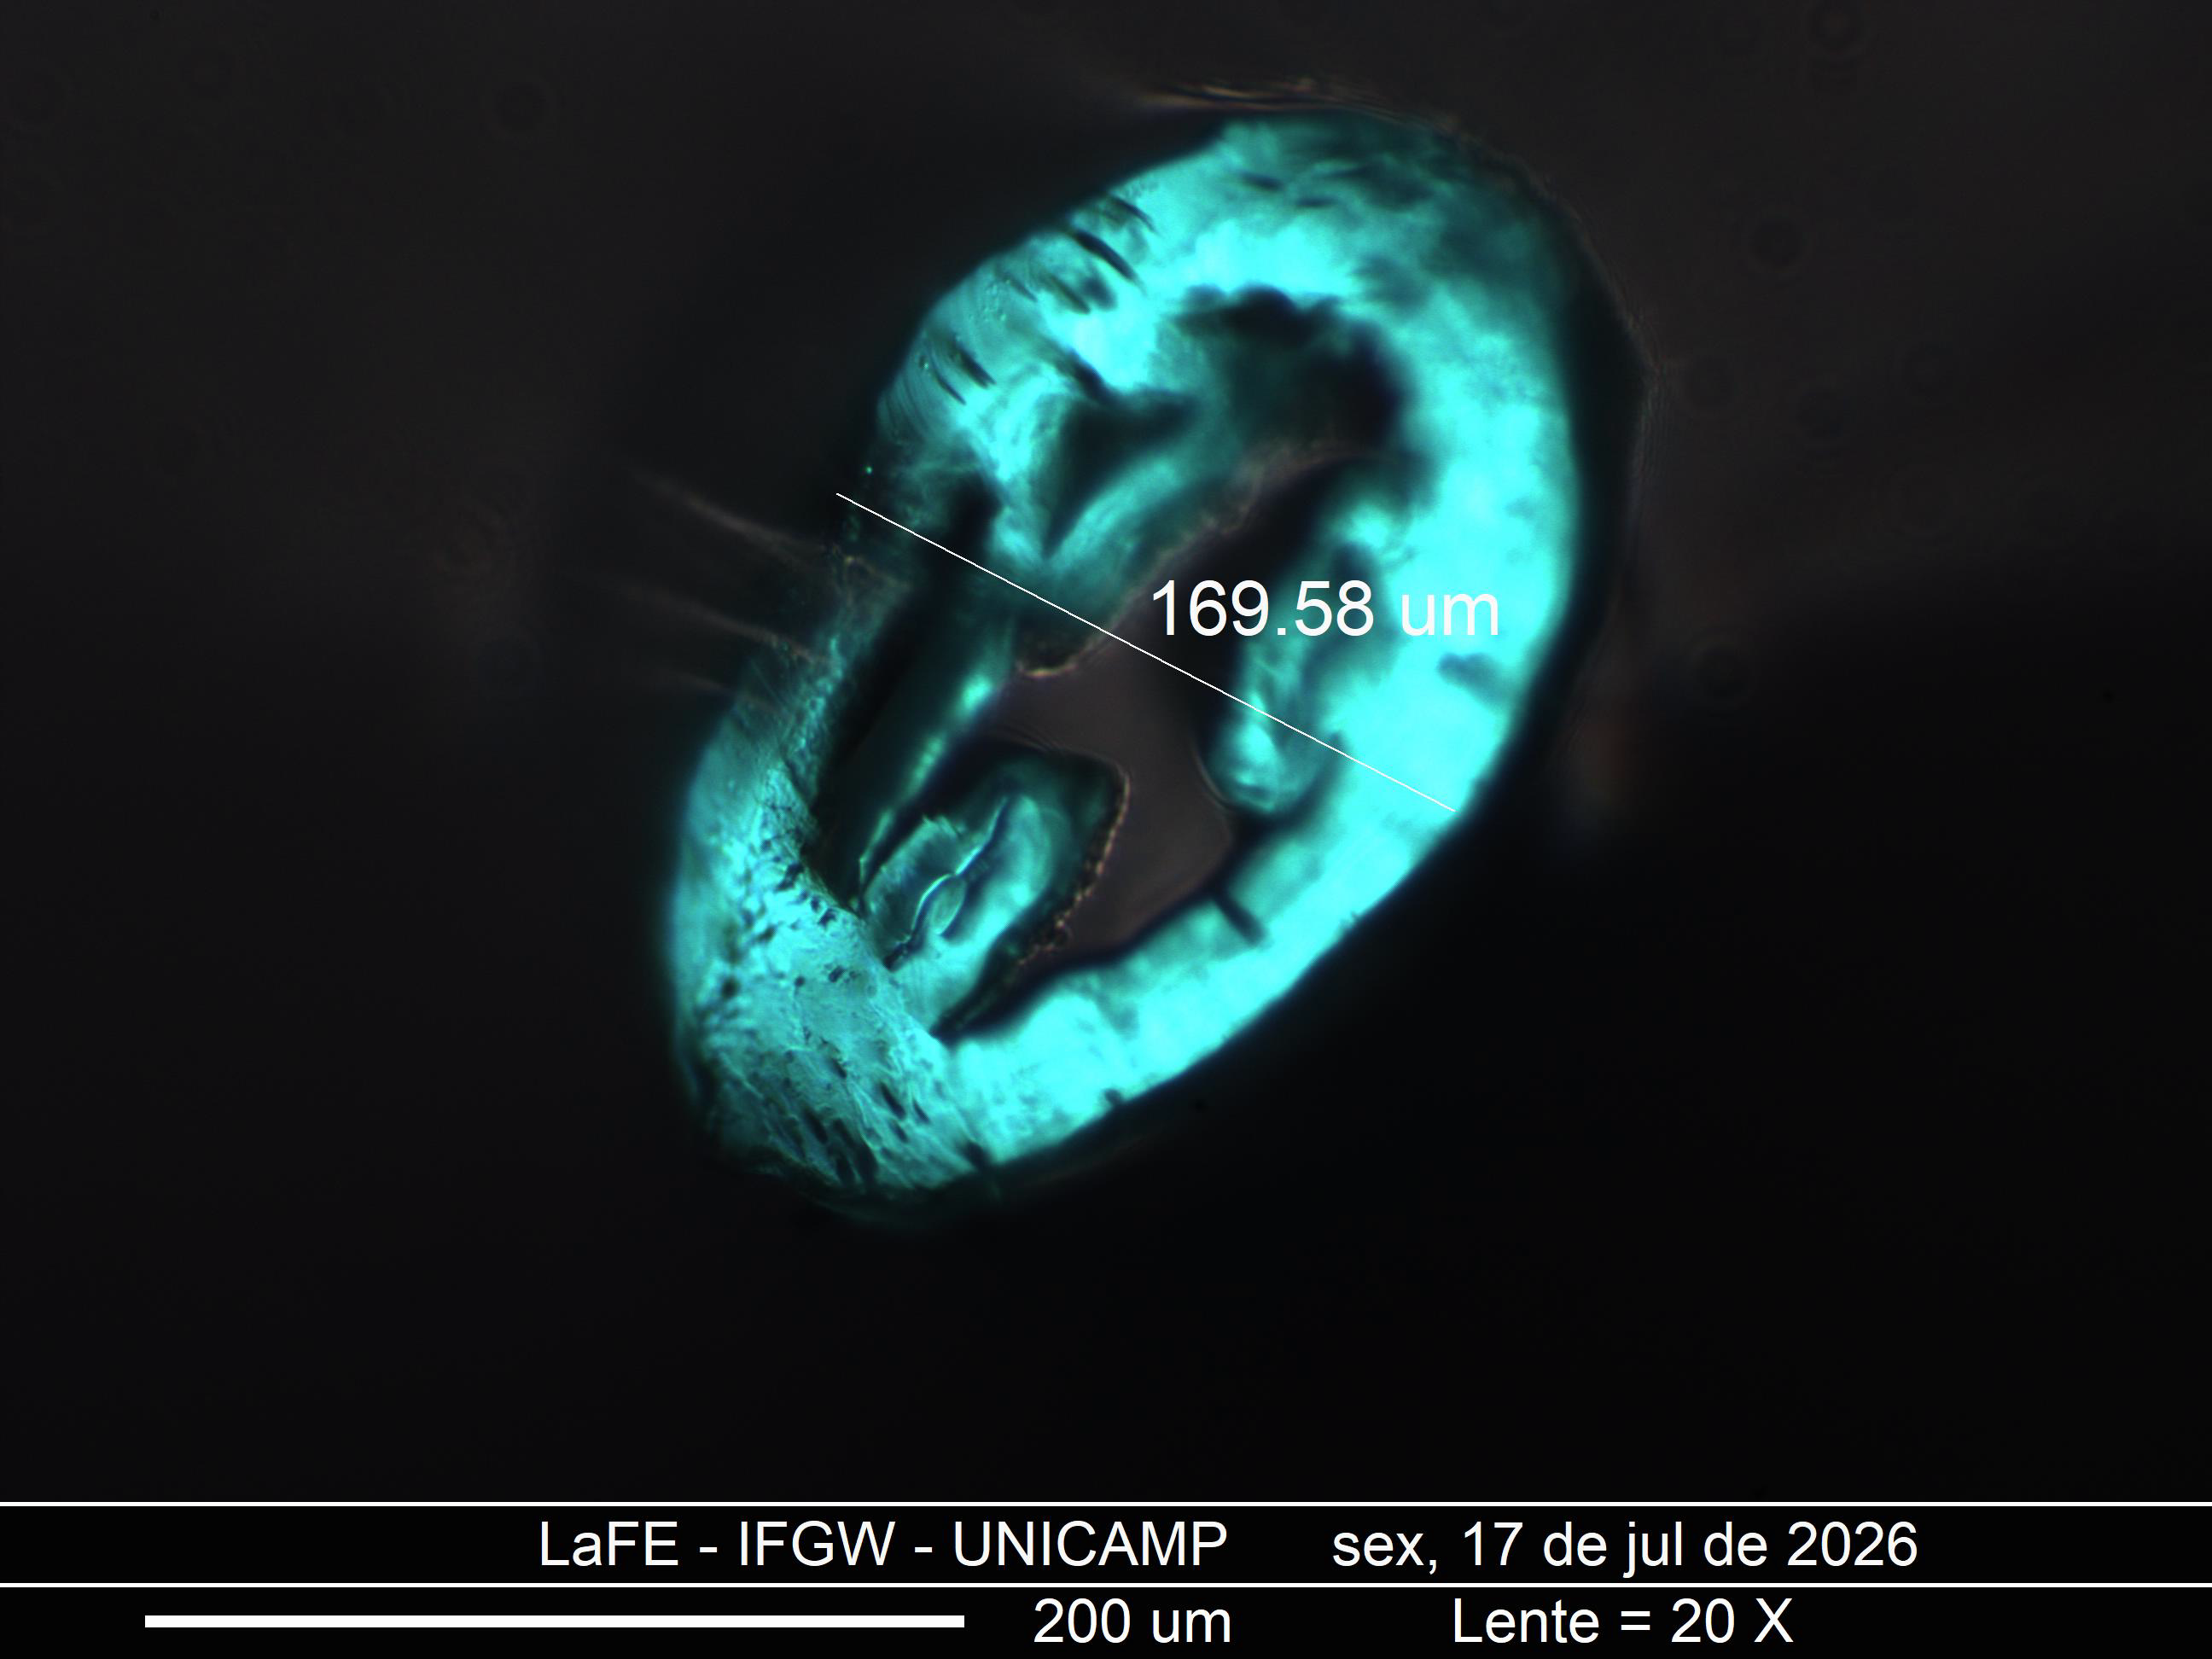
\includegraphics[width=0.45\linewidth]{Banda_B.png}
    \caption{Micrografia da banda B.}
    \label{fig:micrografia_banda_B}
  \end{figure}

  \begin{table}[H]
    \centering
	  \begin{tabular}{c|c|c|c|}	
		  \multirow{2}{*}{\textbf{Medida}} & \multicolumn{3}{c|}{Medidas relativas} \\ 
      & Inicial & M1 & M2 \\
		  \hline
		  $\phi_{out}$ & 1.000 & 1.0000 & 1.0000 \\
		  $L_{out}$ & 0.167 & 0.195 & 0.197 \\
      $\phi_{in}$ & 0.097 & 0.262 & 0.257 \\
		  $L_{in}$ & 0.040 & 0.086 & 0.077 \\
      $d_{int}$ & 0.067 & 0.128 & 0.131
	  \end{tabular}
	  \caption{Medidas na fibra produzida.}
	  \label{tab:medidas_finais}
  \end{table}

  \begin{figure}[H]
    \centering
    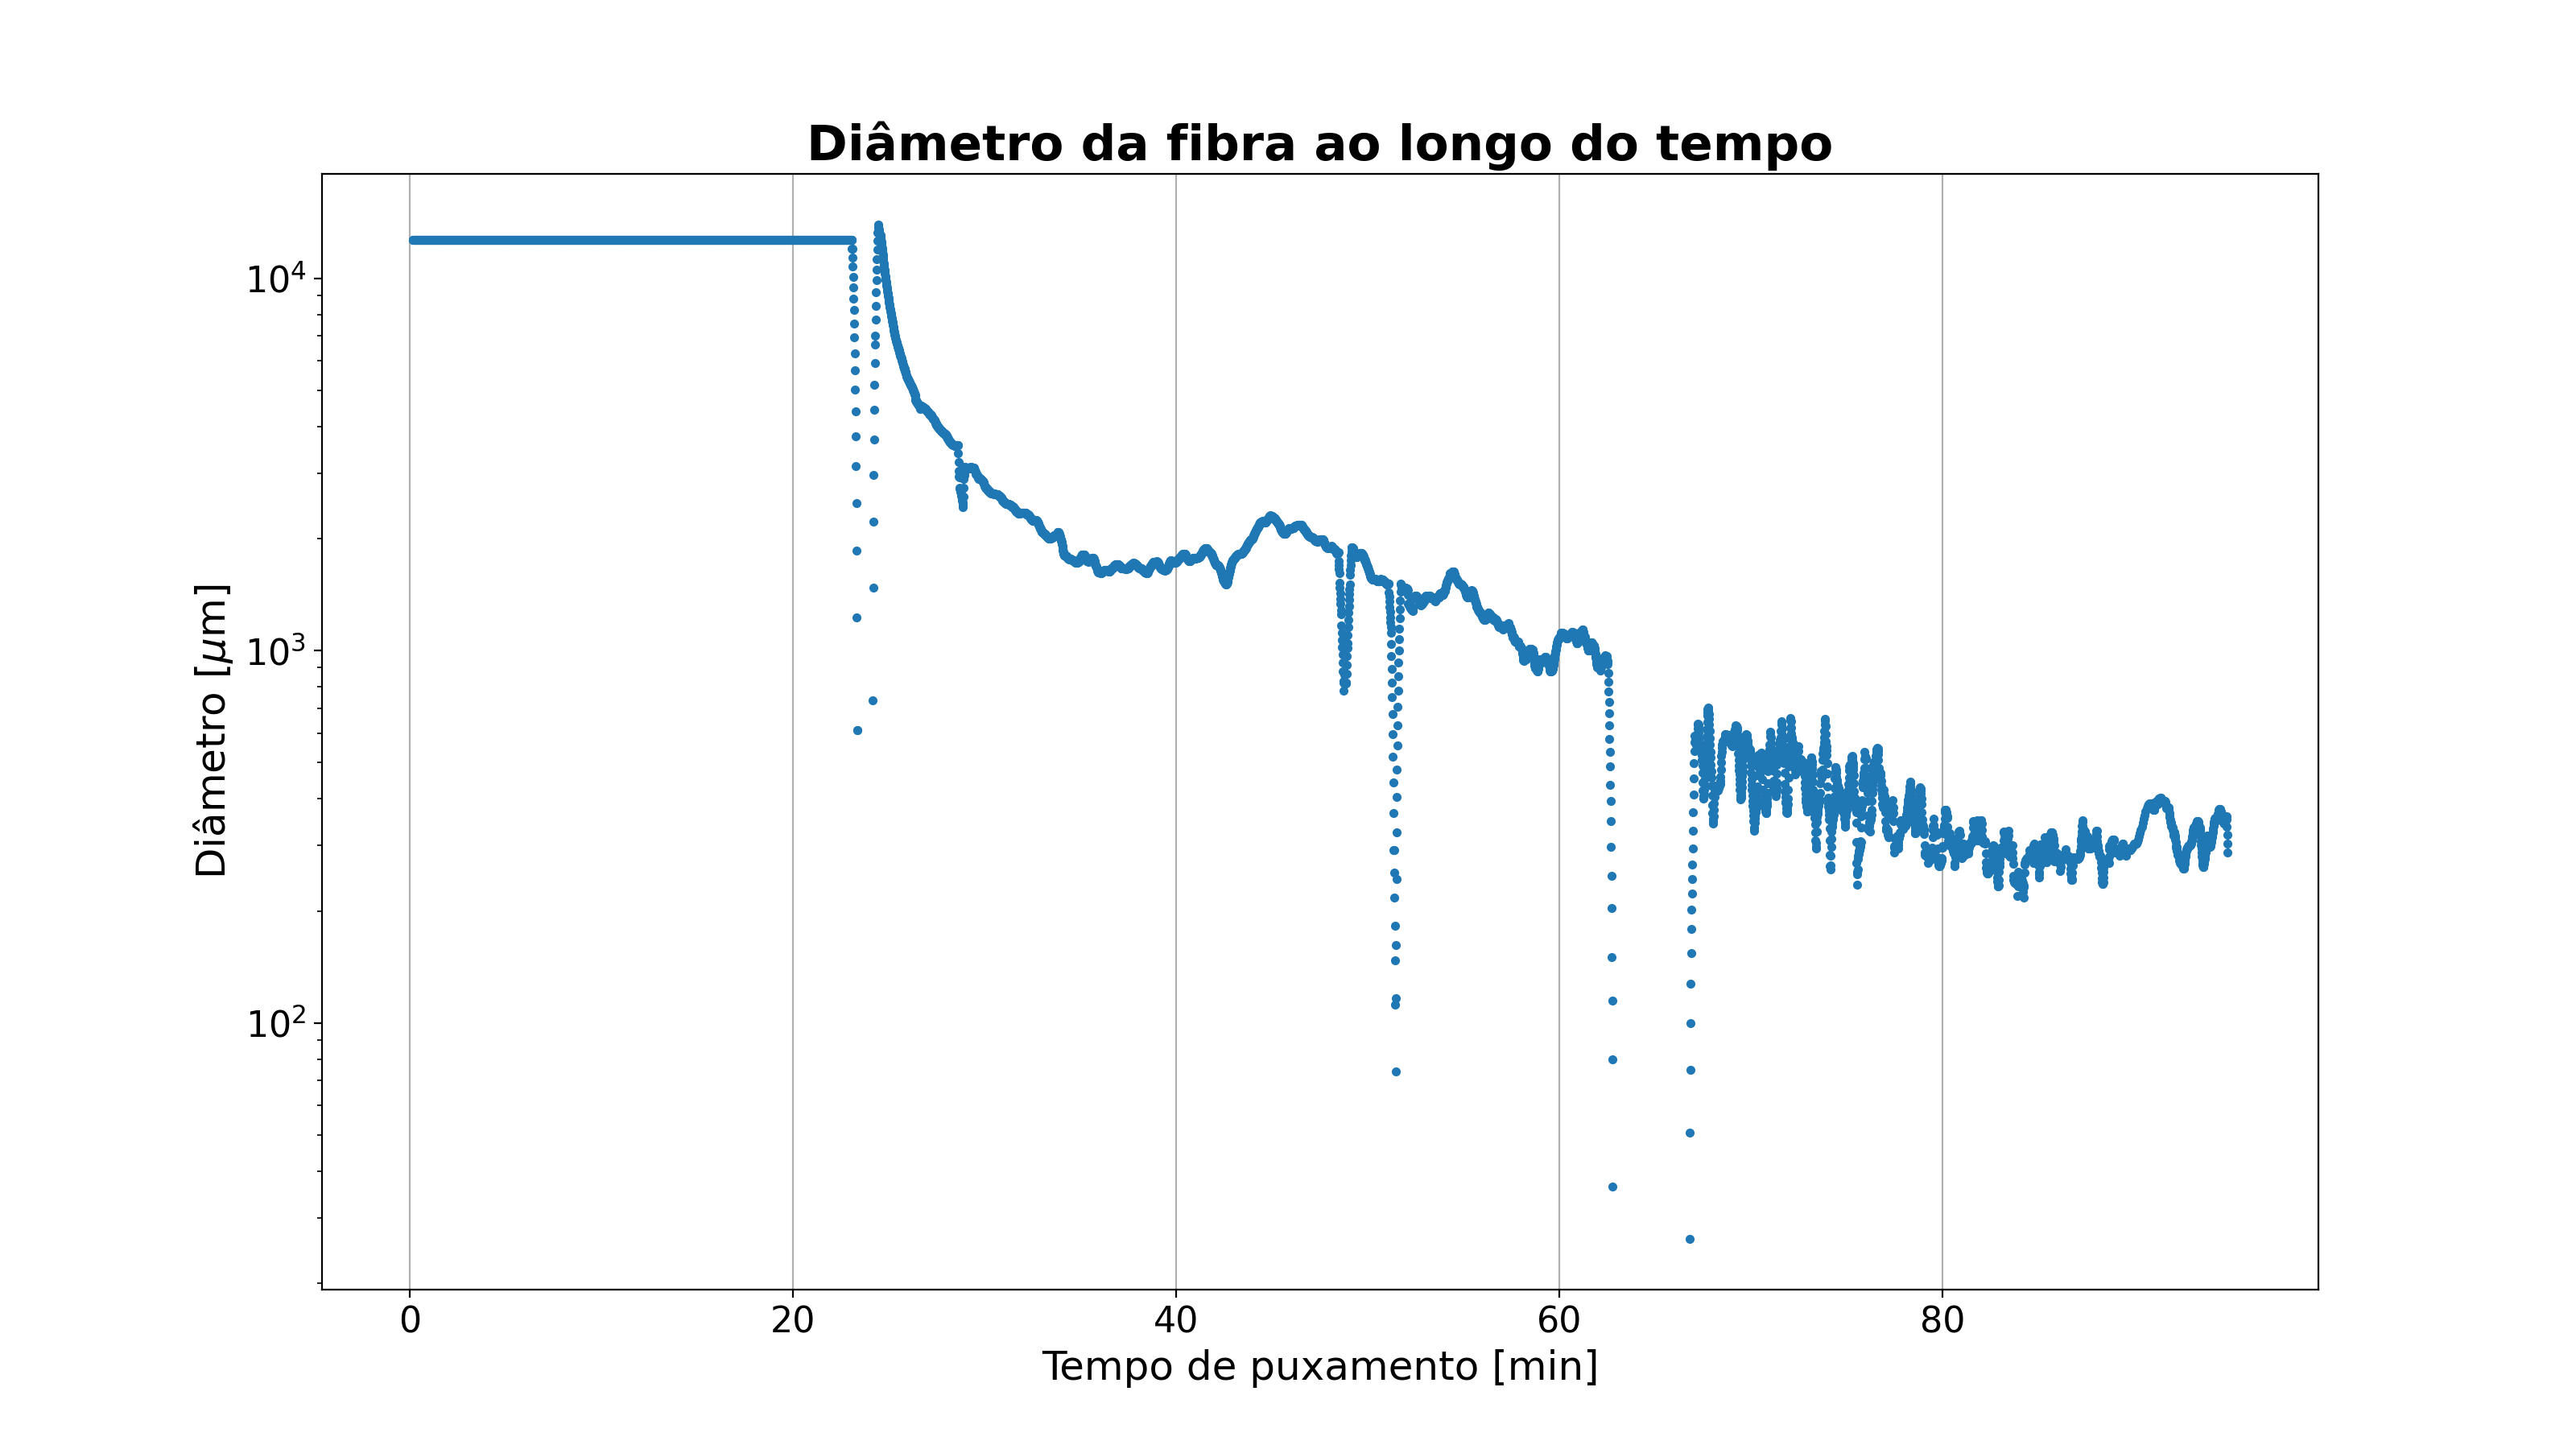
\includegraphics[width=0.9\linewidth]{Diametro.png}
    \caption{Diâmetro medido no Zumbach ao longo do puxamento.}
    \label{fig:grafico_diametros}    
  \end{figure}


\end{document}
